% --- ETUDE DE CAS ---
\section*{AAV}
\addcontentsline{toc}{section}{AAV}
\begin{itemize}
  \item [4] Analyser de manière holistique la sécurité du S.I.
  \item [2] Expliquer le principe de Zone Démilitarisée (DMZ)
  \item [4] Sélectionner le filtrage réseau adapté
  \item [3] Administrer un proxy
  \item [1] Rappeler le cadre légal
  \item [3] Préparer et configurer un pare-feu
  \item [3] Relier les outils de sécurité à l'annuaire du S.I.
\end{itemize}

\section*{Étude de cas: Sécurité et filtrage }
\addcontentsline{toc}{section}{Étude de cas: Sécurité et filtrage }

\subsection*{Mots clés}
\phantomsection
\addcontentsline{toc}{subsection}{Mots clés}
\begin{itemize}
  \item IDPS
  \item DMZ
  \item Proxy 
  \item Pare-feu
  \item UTM
  \item ACL 
  \item DDoS
  \item PSSI 
  \item SOC 
  \item IDS/IPS 
  \item Filtrage 
  \item Vecteur d'attaque
\end{itemize}

\subsection*{Contexte}
\phantomsection
\addcontentsline{toc}{subsection}{Contexte}
Léo travaille actuellement sur un projet de sauvegarde et de sécurisation des données vers le Cloud. L’arrivée d’un technicien réseau pour installer un nouveau pare-feu avec IDPS et un proxy l’amène à réfléchir à l’impact de son projet sur la DMZ, les règles de filtrage et la PSSI du SI.

\subsection*{Problématique}
\phantomsection
\addcontentsline{toc}{subsection}{Problématique}
Comment améliorer la sécurisation des flux de données entre le SI, la DMZ et le Cloud tout en garantissant un filtrage réseau adapté et l’efficacité du proxy et du pare-feu ?

\subsection*{Contraintes}
\phantomsection
\addcontentsline{toc}{subsection}{Contraintes}
\begin{itemize}
  \item Infrastructure
  \item Respect de la PSSI
  \item Déployer un nouveau pare-feu
  \item IDS-IPS
\end{itemize}

\subsection*{Généralisation}
\phantomsection
\addcontentsline{toc}{subsection}{Généralisation}
\begin{itemize}
  \item Sécurité Réseau 
  \item Filtrage Réseau
\end{itemize}

\subsection*{Livrables}
\phantomsection
\addcontentsline{toc}{subsection}{Livrables}
\begin{itemize}
  \item Rapport intrégrant la partie de filtrage (ACL, architecture), le pare-feu, proxy
  \item Déterminer la DMZ et la mettre en place
\end{itemize}

\subsection*{Pistes de solutions}
\phantomsection
\addcontentsline{toc}{subsection}{Pistes de solutions}
\begin{itemize}
  \item Architecture Réseau 
  \item Filtrage 
  \item Logique ACL
  \item Rôles spécifiques d'un Pare-feu, d'un Proxy et d'un IDPS/UTM.
  \item Cadre légal
\end{itemize}

\newpage

\subsection*{Plan d'action}
\phantomsection
\addcontentsline{toc}{subsection}{Plan d'action}
\begin{itemize}
  \item Définir les mots clés (DMZ, Proxy, Firewall, IDPS, etc.).
  \item Analyser l'architecture existante de BERRIA et situer la DMZ.
  \item Faire l’inventaire des ACL
  \item Déterminer les ACL nécessaire
  \item Lister les flux réseaux requis pour le projet Cloud/Sauvegarde (ports TCP/UDP).
  \item Définir les règles de filtrage (ACL) nécessaires sur le pare-feu.
  \item Configurer le rôle du Proxy dans l'infrastructure.
  \item Évaluer les risques et l’impact sur la DMZ
  \item Rédiger la partie filtrage du rapport et compléter l'exercice "Corbeille".
\end{itemize}

\clearpage
\section*{Démarche~: Sécurité et filtrage }
\addcontentsline{toc}{section}{Démarche~: Sécurité et filtrage }

\subsection*{Définition: Mots clés}
\phantomsection
\addcontentsline{toc}{subsection}{Définition: Mots clés}

\noindent \textbf{IDPS (Intrusion Detection and Prevention System)}:\\
Un IDPS est un système chargé de détecter et, si nécessaire, de bloquer en temps réel les tentatives d’intrusion ou les comportements anormaux dans un réseau. Il s’appuie à la fois sur des signatures (attaques connues) et sur l’analyse comportementale (écarts par rapport à la norme).\\
L’IDS observe et alerte, tandis que l’IPS peut intervenir directement en coupant ou modifiant le trafic. Bien positionné dans l’architecture réseau, un IDPS permet de repérer précocement les phases de reconnaissance, les exfiltrations et les attaques actives.

\medskip

\noindent \textbf{DMZ (DeMilitarized Zone)}:\\
La DMZ est une zone tampon située entre Internet et le réseau interne. On y place les services destinés au public (site web, serveur mail, DNS, portail VPN) afin qu’une compromission éventuelle n’ouvre pas la porte au reste du système d’information.\\
L’idée centrale est le cloisonnement strict : les flux sont limités et contrôlés, et la DMZ agit comme un espace séparé qui protège le cœur du réseau.

\medskip

\noindent \textbf{Proxy}:\\
Un proxy est un serveur intermédiaire qui gère les communications entre les utilisateurs internes et Internet. Il peut filtrer l’accès à certains sites, mettre en cache les contenus pour optimiser les performances, appliquer des politiques de sécurité, enregistrer les actions et masquer les adresses internes.\\
C’est un point de contrôle essentiel pour encadrer et surveiller la navigation web.

\medskip

\noindent \textbf{Pare-feu (Firewall)}:\\
Le pare-feu est l’outil central de la défense périmétrique. Il contrôle les flux réseau selon des règles précises : adresses IP, ports, protocoles et parfois types d’applications. Les pare-feux modernes (NGFW) inspectent aussi le contenu des paquets, intègrent le contrôle applicatif, le VPN ou encore des mécanismes de prévention d’intrusions.\\
Un firewall efficace est celui dont les règles sont claires, limitées et régulièrement maintenues.

\medskip

\noindent \textbf{1. Pare‑feu de filtrage (niveau réseau / packet‑filtering, stateless ou stateful)}:\\
Un pare‑feu de filtrage opère principalement sur les en‑têtes réseau : adresses IP, ports et protocoles.  
- Stateless : examine chaque paquet indépendamment (rapide, simple, moins contextuel).  
- Stateful : conserve l'état des connexions (suivi des sessions TCP/UDP), autorise les réponses légitimes et bloque les paquets hors contexte.  
Avantages : faible latence, simple à déployer. Limites : visibilité limitée au contenu, moins efficace contre attaques applicatives.

\newpage

\noindent \textbf{2. Pare‑feu applicatif (niveau application / proxy ou NGFW)}:\\
Travaille au niveau applicatif (HTTP, SMTP, DNS, etc.) : peut analyser le contenu, les URLs, les en‑têtes applicatifs et effectuer inspection SSL/TLS, DLP, contrôle d'applications et filtrage par utilisateur. Les NGFW intègrent IDS/IPS, antivirus et fonctions de proxys.  
Avantages : contrôle granulaire, meilleure détection des menaces applicatives et exfiltration. Limites : plus coûteux, impact sur la latence et nécessité de gestion des certificats pour l'inspection TLS.

\textbf{Solutions commerciales pour pare‑feu}
\begin{itemize}
  \item Palo Alto Networks
  \item Fortinet (FortiGate)
  \item Check Point
  \item Cisco Firepower
  \item Juniper SRX
  \item pfSense / OPNsense (open‑source)
\end{itemize}

\medskip

\noindent \textbf{UTM (Unified Threat Management)}:\\
Un UTM regroupe dans un seul équipement plusieurs fonctions de sécurité : pare-feu, IPS, antivirus, filtrage web, gestion VPN, anti-spam, etc. Cette approche simplifie la gestion et offre une vision unifiée de la sécurité.\\
L’inconvénient est qu’un UTM concentre tous les services critiques : s’il tombe, tout tombe. Il peut aussi devenir un goulot d’étranglement si on active trop de modules.

\medskip

\noindent \textbf{ACL (Access Control List)}:\\
Une ACL est une liste de règles permettant d’autoriser ou de refuser l’accès à certaines ressources ou à certains flux réseau. Elles peuvent s’appliquer à un routeur, un pare-feu, un commutateur de niveau 3 ou même à un système de fichiers.\\
Les ACL sont un outil puissant mais sensible : une règle trop permissive ou mal ordonnée peut annuler toute une architecture de sécurité.

\medskip

\noindent \textbf{DDoS (Distributed Denial of Service)}:\\
Une attaque DDoS vise à rendre un service indisponible en l’inondant de requêtes provenant de nombreuses machines compromises. Elle peut saturer la bande passante, épuiser les ressources d’un serveur ou bloquer une application spécifique.\\
La défense repose sur la détection précoce, le filtrage, le découpage de charge (load balancing), le recours à des CDN ou à des solutions anti-DDoS spécialisées.

\medskip

\noindent \textbf{PSSI (Politique de Sécurité des Systèmes d’Information)}:\\
La PSSI définit les objectifs, les règles et les responsabilités en matière de sécurité au sein d’une organisation. Elle fixe le cadre global : gestion des risques, accès, sauvegardes, sensibilisation, conformité réglementaire et réponse aux incidents.\\
C’est le document de référence à partir duquel toutes les mesures concrètes de sécurité doivent être alignées.

\newpage

\noindent \textbf{SOC (Security Operation Center)}:\\
Le SOC est l’équipe (ou le service) chargée de surveiller le système d’information en continu. Il collecte et analyse les journaux, détecte les activités suspectes, déclenche les procédures de réponse aux incidents et mène des investigations.\\
Un SOC mature combine outils avancés (SIEM, EDR, XDR), expertise humaine et veille permanente sur les menaces.

\medskip

\noindent \textbf{IDS / IPS}:\\
Un IDS détecte les intrusions en analysant le trafic ou les actions exécutées sur un système ; il alerte mais n’agit pas. Un IPS va plus loin : il bloque ou modifie le trafic dangereux dès qu’il est détecté.\\
En pratique, IDS et IPS sont souvent complémentaires : l’un observe, l’autre protège.

\medskip

\noindent \textbf{Filtrage}:\\
Le filtrage consiste à contrôler ce qui a le droit de passer : flux réseau, applications, adresses IP, URLs, protocoles ou encore utilisateurs. Il s’effectue au niveau des pare-feux, des proxies, des switches ou des outils applicatifs (WAF, par exemple).\\
C’est le principe fondamental de réduction de la surface d’attaque.

\medskip

\noindent \textbf{Vecteur d’attaque}:\\
Un vecteur d’attaque est la voie utilisée par un pirate pour entrer ou exploiter un système. Il peut s’agir d’un email de phishing, d’une faille logicielle, d’un service exposé sans protection, d’identifiants volés ou encore d’une manipulation humaine (ingénierie sociale).\\
Comprendre les vecteurs d’attaque permet d’anticiper et de réduire les scénarios d’intrusion les plus probables.

\newpage

\section*{Corbeille: Sécurité et filtrage}
\addcontentsline{toc}{section}{Corbeille: Sécurité et filtrage}

\noindent Cette corbeille d'exercices est la suite du workshop « Sécurité/Filtrage » et aborde les points suivants :
\begin{itemize}
  \item Administration déléguée du pare-feu à l'aide de l'authentification sur Active Directory.
  \item Mise en place d'un proxy transparent avec Squid.
  \item Mise en place d'un filtre web avec Squidguard.
\end{itemize}

\subsection*{Configuration nécessaire}
\phantomsection
\addcontentsline{toc}{subsection}{Configuration nécessaire}
\noindent Le plan d'adressage proposé peut être adapté à votre propre Plan s'adressage. Vous devez être capable de vous adapter.

\begin{center}
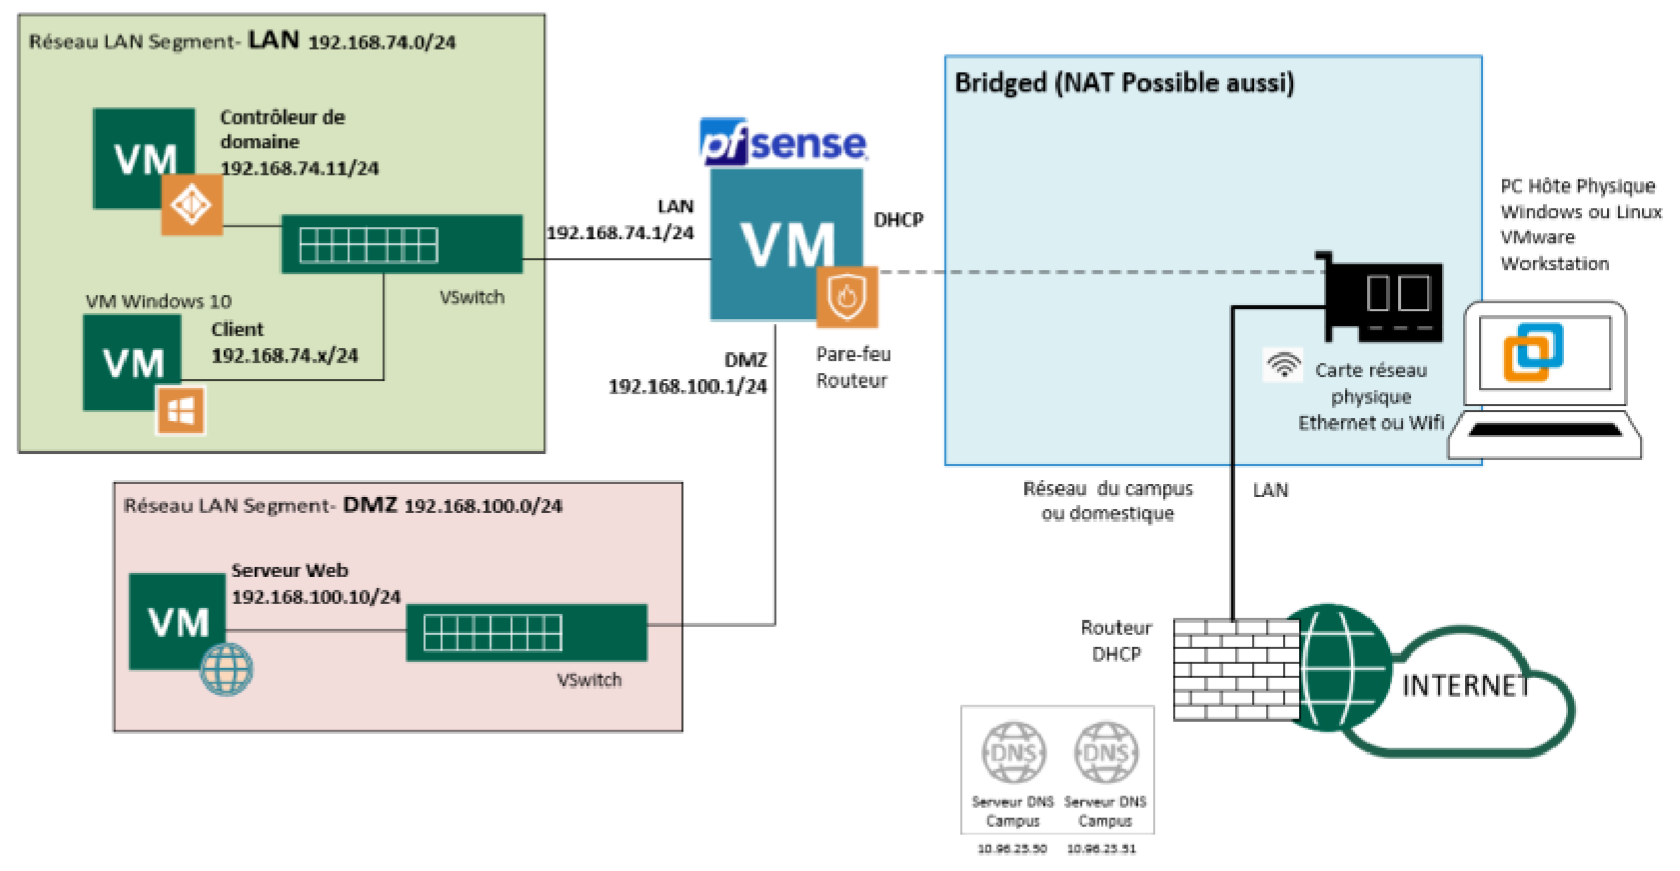
\includegraphics[width=0.8\textwidth]{contents/img/configuration.png}
\end{center}

\noindent Pour rappel, la topologie déjà configurée lors du workshop «Sécurité/Filtrage» est constituée de 4 machines virtuelles.
Dans le cadre de cette corbeille vous n'avez pas besoin du serveur web en DMZ. Vous pouvez l'éteindre pour avoir plus de
ressources.

\noindent Vous pouvez faire toute la corbeille en utilisant uniquement le serveur Windows 2022 et donc éteindre le PC virtuel W10 ou 11.
C'est à votre convenance.

\textit{Nécessaire}
\begin{itemize}
  \item Une machine sous pfSense (Firewall) avec 3 interfaces réseau fonctionnelle
\end{itemize}

\textit{Sur le LAN :}
\begin{itemize}
  \item Une machine sous WS 2022 rôle domain controller et serveur DNS
\end{itemize}

\textit{Optionnel}
\begin{itemize}
  \item Une machine sous Windows 10 ou 11 (rôle membre du domaine)
\end{itemize}

\subsection*{PARTIE 1 - Administration déléguée du pare-feu}
\phantomsection
\addcontentsline{toc}{subsection}{PARTIE 1 - Administration déléguée du pare-feu}

\noindent pfSense permet une connexion à un annuaire \textbf{LDAP}, notamment Active Directory, pour déléguer l'administration du pare-feu à certains utilisateurs. Vous allez voir dans cette partie comment l'implémenter tout en attribuant et/ou limitant certains accès en fonction des groupes AD correspondants.

\begin{itemize}
  \item Vous aller créer dans votre domaine Active Directory créé lors d'un Workshop précédent, une Unité d'Organisation qui contiendra des comptes utilisateurs administrateurs du pare-feu avec différents rôles
  \item Vous allez ensuite paramétrer pfSense pour utiliser ces comptes à l'aide de leur DN.
\end{itemize}

\noindent Vous n'avez pas besoin de votre VM PC W10 ou 11 pour travailler sur cette partie

\vspace{1cm}

\noindent \textbf{Création de comptes administrateurs pfsense dans Active Directory}

\begin{itemize}
  \item Connectez-vous sur votre serveur Windows 2022 contrôleur de domaine.
  \item Vous aller créer une OU dans votre domaine AD, que vous allez nommer ‘IT'.
  \item Vous pouvez utiliser le Centre d'administration Active Directory ou Utilisateurs et ordinateurs Active Directory
  \item Vous allez créer deux utilisateurs : « admin\_junior » et « admin\_senior » et un simple utilisateur « pfsense.connect »
  \item Vous pouvez le faire via deux méthodes : Interface GUI (graphique) et Commandes Powershell.
\end{itemize}

\vspace{0.5cm}

\noindent Question~: \textbf{Créer les utilisateurs admin\_junior et pfsense.connect avec l'interface graphique}

\noindent A l'intérieur de l'OU « IT » créée, vous cliquez sur « Create a New User in the current container», et vous entrez les informations relatives à l'utilisateur.

\noindent Très important : N'oubliez pas le mot de passe donné à « admin\_junior »

\vspace{0.5cm}

\noindent Question~: \textbf{Créer l'utilisateur admin\_senior en utilisant powershell}

\vspace{0.5cm}

\begin{verbatim}
  $password="" | ConvertTo-SecureString -AsPlainText -Force
  New-ADUser -Name "admin_senior" -GivenName "Admin" -Surname 
  "Senior" -SamAccountName "admin_senior" -UserPrincipalName "
\end{verbatim}

\newpage

\noindent Question~: \textbf{Utilisez La méthode GUI pour créer le groupe « GG\_Junior » dans l'OU « IT ».}

\noindent A l'intérieur de l'OU « IT » créée, vous cliquez sur « Create a New Group in the current container », et vous entrez les informations relatives au groupe.

\vspace{0.5cm}

\noindent Question~: \textbf{Ajouter l'utilisateur « admin\_senior » au groupe « GG\_Senior » en utilisant powershell}

\vspace{0.5cm}

\begin{verbatim}
  Add-ADGroupMember -Identity "GG_Senior" -Members "admin_senior"
\end{verbatim}

\vspace{1cm}

\noindent \textbf{Récupération du Distinguished Name (DN) de l'OU, des Utilisateurs et des
Groupes créés}

\noindent Le \textbf{Distinguished Name (DN)} est un identifiant unique utilisé principalement dans les certificats numériques (X.509) et dans \textbf{les annuaires LDAP / Active Directory} pour désigner de manière précise une entité (utilisateur, serveur, organisation…).

\noindent C’est un peu l’équivalent d’un chemin absolu dans un système de fichiers.

\noindent Il faut pouvoir identifier de façon claire, unique et hiérarchique chaque objet dans une structure d'annuaire

\vspace{0.5cm}

\begin{center}
{\small
\begin{tabular}{|l|l|p{4cm}|l|}
\hline
Abréviation & Nom complet & Rôle dans le DN & Exemple \\ \hline
CN & Common Name & Nom de l’objet (utilisateur, groupe, ordinateur, etc.) & CN=Alan Turing \\ \hline
OU & Organizational Unit & Unité d’organisation (contenant logique d'objets dans l'annuaire) & OU=Comptabilité \\ \hline
DC & Domain Component & Élément du nom de domaine utilisé pour construire le DN & DC=entreprise, DC=local \\ \hline
\end{tabular}
}
\end{center}

\vspace{0.5cm}

\begin{itemize}
  \item L’ordre est \textbf{inversé} par rapport à la hiérarchie logique (du plus spécifique au plus général).
  \item Les DN sont \textbf{uniques} dans l’annuaire
  \item Tous les objets AD (y compris les groupes, ordinateurs, imprimantes) ont un \textbf{DN}.
  \item Le DN complet sert dans les scripts PowerShell, les requêtes LDAP, les outils d’administration.
\end{itemize}

\newpage

\noindent Question~: \textbf{Savez-vous retrouver le DN des éléments créés en utilisant POWERSHELL ?}

\begin{itemize}
  \item OU : IT
  \item Utilisateurs : admin\_senior et admin\_junior
  \item Groupes : GG\_Senior et GG\_Junior
\end{itemize}

\vspace{0.5cm}

\begin{verbatim}
  PS C:\Users\Administrateur> Get-ADUser -Identity "admin_senior"
   | Select-Object DistinguishedName
  
  DistinguishedName
  -----------------
  CN=admin_senior,OU=IT,DC=lab,DC=intra
  PS C:\Users\Administrateur> Get-ADGroup -Identity "GG_Senior"
   | Select-Object DistinguishedName
 
  DistinguishedName
  -----------------
  CN=GG_Senior,OU=IT,DC=lab,DC=intra
  PS C:\Users\Administrateur> Get-ADOrganizationalUnit -Filter
   "Name -eq 'IT'" | Select-Object DistinguishedName
  
  DistinguishedName
  -----------------
  OU=IT,DC=lab,DC=intra
\end{verbatim}

\vspace{1cm}

\noindent Question~: \textbf{Savez-vous retrouver le DN des éléments créés via l'INTERFACE GRAPHIQUE ?}

\noindent Vous devez utiliser les fonctionnalités avancées de la console Utilisateurs et ordinateurs Active Directory

\begin{itemize}
  \item Ouvrer \textbf{Utilisateurs et ordinateurs Active Directory} (ADUC).
  \item Activer l’option : \textbf{Affichage > Fonctionnalités avancées}.
  \item Cliquer droit sur un utilisateur > \textbf{Propriétés}.
  \item Onglet \textbf{Éditeur d’attributs} (ou "Attribute Editor").
  \item Chercher \textbf{distinguishedName}
\end{itemize}

\vspace{1cm}

[ ... La suite de la corbeille est disponible dans le fichier séparé \\ corbeille\_securite\_filtrage.tex ... ]

\newpage

\section*{Analyse et résolution: Sécurité et filtrage}
\addcontentsline{toc}{section}{Analyse et résolution: Sécurité et filtrage}

\subsection*{Analyser l'architecture existante de BERRIA et situer la DMZ}
\phantomsection
\addcontentsline{toc}{subsection}{Analyser l'architecture existante de BERRIA et situer la DMZ}

\noindent L'architecture réseau de BERRIA suit un modèle de sécurité en couches avec trois zones distinctes :

\medskip

\noindent \textbf{Zone Internet (non maîtrisée)} :\\
Cette zone représente l'extérieur, source de menaces potentielles. Tout trafic en provenance de cette zone est considéré comme non fiable et doit être filtré et inspecté.

\medskip

\noindent \textbf{DMZ (Zone Démilitarisée)} :\\
Positionnée entre Internet et le réseau interne, la DMZ héberge les services accessibles au public :
\begin{itemize}
  \item Site portail de l'ERP (interface web publique)
  \item Serveur de messagerie (SMTP, IMAP)
  \item Serveurs DNS publics
  \item Éventuellement : serveur VPN, serveurs web institutionnels
\end{itemize}

\noindent Cette zone est protégée par le pare-feu principal côté Internet, mais reste isolée du réseau interne par un second niveau de filtrage. En cas de compromission d'un serveur dans la DMZ, l'attaquant ne dispose pas d'un accès direct au cœur du système d'information.

\medskip

\noindent \textbf{Réseau interne (LAN)} :\\
C'est le cœur du SI de BERRIA, hébergeant :
\begin{itemize}
  \item Les postes de travail des employés
  \item Les serveurs métiers (ERP, bases de données, applications internes)
  \item Les ressources de stockage et de sauvegarde
  \item L'Active Directory et les services d'authentification
\end{itemize}

\noindent Le pare-feu contrôle strictement les flux entre le LAN et la DMZ. Seuls les flux légitimes et nécessaires sont autorisés (par exemple : connexion du serveur web DMZ vers la base de données interne sur des ports spécifiques).

\newpage

\noindent \textbf{Flux de sécurité} :\\
Le nouveau déploiement inclut :
\begin{itemize}
  \item Un pare-feu avec IDPS pour détecter et bloquer les intrusions en temps réel
  \item Un proxy pour filtrer et contrôler les accès web sortants depuis le LAN
  \item Un UTM (Unified Threat Management) intégrant IDS/IPS, antivirus et filtrage
  \item Une supervision centralisée vers le SOC pour l'analyse des événements
\end{itemize}

\noindent Cette architecture permet d'appliquer le principe de défense en profondeur : plusieurs couches de sécurité successives limitent la propagation d'une attaque et multiplient les chances de détection.

\subsection*{Faire l'inventaire des ACL}
\phantomsection
\addcontentsline{toc}{subsection}{Faire l'inventaire des ACL}

\noindent L'inventaire des ACL existantes chez BERRIA permet d'identifier les points de contrôle actuels et de comprendre comment les flux sont régulés dans l'architecture réseau. Cet inventaire se structure par équipement et par zone.

\medskip

\noindent \textbf{1. ACL sur le routeur principal (Internet $\leftrightarrow$ Pare-feu)} :\\
\begin{itemize}
  \item \textbf{ACL-INTERNET-IN} : Filtre le trafic entrant depuis Internet
  \begin{itemize}
    \item Bloque les adresses IP privées (RFC 1918) en provenance d'Internet
    \item Bloque les paquets avec source spoofée
    \item Autorise uniquement les connexions établies (stateful)
    \item Limite les flux ICMP (anti-scan, anti-reconnaissance)
  \end{itemize}
  
  \item \textbf{ACL-INTERNET-OUT} : Contrôle le trafic sortant vers Internet
  \begin{itemize}
    \item Autorise les flux sortants légitimes depuis la DMZ et le LAN
    \item Bloque les protocoles non autorisés (Telnet, FTP non sécurisé)
    \item Limite la bande passante par type de flux
  \end{itemize}
\end{itemize}

\medskip

\noindent \textbf{2. ACL sur le pare-feu principal (Internet $\leftrightarrow$ DMZ)} :\\
\begin{itemize}
  \item \textbf{ACL-DMZ-IN} : Autorise l'accès public aux services exposés
  \begin{itemize}
    \item HTTP/HTTPS (80, 443) vers serveur web portail ERP
    \item SMTP (25, 587) vers serveur de messagerie
    \item DNS (53 UDP/TCP) vers serveurs DNS publics
    \item VPN (500, 4500 UDP pour IPsec) si applicable
    \item Tous les autres flux sont refusés par défaut (deny all)
  \end{itemize}
  
  \item \textbf{ACL-DMZ-OUT} : Contrôle les flux sortants depuis la DMZ
  \begin{itemize}
    \item Autorise les réponses aux connexions établies
    \item Autorise les mises à jour système (HTTPS vers dépôts officiels)
    \item Autorise DNS sortant pour résolution de noms
    \item Autorise SMTP sortant pour envoi de mails
    \item Bloque toute tentative de connexion vers le LAN interne
  \end{itemize}
\end{itemize}

\medskip

\noindent \textbf{3. ACL sur le pare-feu interne (DMZ $\leftrightarrow$ LAN)} :\\
\begin{itemize}
  \item \textbf{ACL-LAN-TO-DMZ} : Autorise le LAN à administrer et utiliser la DMZ
  \begin{itemize}
    \item SSH (22) depuis postes d'administration uniquement
    \item RDP (3389) pour administration Windows
    \item HTTPS (443) vers portail ERP pour utilisateurs internes
    \item Accès base de données (1433 SQL Server, 3306 MySQL, 5432 PostgreSQL) depuis serveurs métiers uniquement
    \item Monitoring (SNMP 161/162, Syslog 514) depuis serveur de supervision
  \end{itemize}
  
  \item \textbf{ACL-DMZ-TO-LAN} : Restreint fortement les accès DMZ vers LAN
  \begin{itemize}
    \item Accès base de données interne depuis serveur web DMZ (ports spécifiques, IP source précise)
    \item Authentification LDAP/AD (389, 636, 88 Kerberos) pour les services DMZ
    \item Accès NTP (123) pour synchronisation horaire
    \item Tous les autres flux sont bloqués (principe du moindre privilège)
  \end{itemize}
\end{itemize}

\medskip

\noindent \textbf{4. ACL sur le pare-feu LAN (Utilisateurs $\leftrightarrow$ Internet)} :\\
\begin{itemize}
  \item \textbf{ACL-LAN-OUT} : Régule les accès Internet depuis le LAN
  \begin{itemize}
    \item HTTP/HTTPS (80, 443) via proxy obligatoire
    \item DNS (53) vers serveurs DNS internes uniquement
    \item SMTP (587) via serveur mail interne
    \item Bloque les accès directs à Internet sans passer par le proxy
    \item Bloque les protocoles à risque (P2P, Tor, proxies anonymes)
  \end{itemize}

  \newpage
  
  \item \textbf{ACL-LAN-INTERNAL} : Segmente le trafic interne
  \begin{itemize}
    \item VLAN utilisateurs : accès aux serveurs métiers, imprimantes, partages
    \item VLAN serveurs : communication inter-serveurs restreinte
    \item VLAN administration : accès complet pour équipe IT
    \item VLAN IoT/imprimantes : isolé du reste du réseau
  \end{itemize}
\end{itemize}

\medskip

\noindent \textbf{5. ACL sur les switches de distribution (segmentation VLAN)} :\\
\begin{itemize}
  \item \textbf{ACL-VLAN} : Contrôle les flux inter-VLAN
  \begin{itemize}
    \item VLAN 10 (utilisateurs) $\rightarrow$ VLAN 20 (serveurs) : autorisé avec filtrage
    \item VLAN 30 (invités) : isolé, accès Internet uniquement via proxy
    \item VLAN 40 (management) : accès SSH/HTTPS aux équipements réseau
    \item VLAN 50 (VoIP) : priorisé (QoS) et isolé des autres VLANs
  \end{itemize}
\end{itemize}

\medskip

\noindent \textbf{6. ACL proxy (filtrage applicatif web)} :\\
\begin{itemize}
  \item \textbf{ACL-PROXY-WEB} : Contrôle l'accès aux sites web
  \begin{itemize}
    \item Liste blanche : sites métiers autorisés
    \item Liste noire : réseaux sociaux, streaming, sites malveillants
    \item Filtrage par catégorie (adultes, jeux, malwares, phishing)
    \item Inspection SSL/TLS pour détecter les menaces dans le trafic chiffré
    \item Journalisation complète pour audit et conformité
  \end{itemize}
\end{itemize}

\medskip

\noindent \textbf{7. ACL pour le projet Cloud/Sauvegarde (à créer)} :\\
Ces ACL devront être ajoutées pour le projet de Léo :
\begin{itemize}
  \item Flux vers solution de sauvegarde Cloud (ports HTTPS 443, protocoles spécifiques)
  \item Authentification et chiffrement des données en transit
  \item Restriction des serveurs autorisés à sauvegarder vers le Cloud
  \item Monitoring et alertes sur les volumes de données transférées
\end{itemize}

\medskip

\noindent \textbf{Constats de l'inventaire} :\\
L'inventaire révèle une architecture de sécurité globalement bien structurée, mais certains points nécessitent attention :
\begin{itemize}
  \item Les ACL entre DMZ et LAN sont critiques et doivent être auditées régulièrement
  \item Le projet Cloud/Sauvegarde nécessite de nouvelles règles spécifiques
  \item Le proxy doit être configuré pour gérer les flux vers les services Cloud
  \item La documentation des ACL doit être maintenue à jour dans la PSSI
\end{itemize}

\newpage

\subsection*{Déterminer les ACL nécessaire}
\phantomsection
\addcontentsline{toc}{subsection}{Déterminer les ACL nécessaire}

Pour le projet de sauvegarde et de sécurisation des données vers le Cloud, Léo doit déterminer les ACL spécifiques qui permettront de sécuriser les flux tout en respectant la PSSI de BERRIA. Cette analyse se base sur les besoins fonctionnels du projet et les contraintes de sécurité.

\medskip

\noindent \textbf{1. ACL-CLOUD-BACKUP-OUT : Flux sortants vers la solution Cloud} :\\
Cette ACL contrôle les connexions depuis le réseau interne vers les services de sauvegarde Cloud.

\begin{itemize}
  \item \textbf{Source} : Serveurs de sauvegarde autorisés (liste IP précise)
  \begin{itemize}
    \item Serveur principal de backup : 10.10.20.10
    \item Serveur secondaire de backup : 10.10.20.11
    \item Pas d'autorisation pour d'autres serveurs ou postes utilisateurs
  \end{itemize}
  
  \item \textbf{Destination} : Adresses IP du fournisseur Cloud (plages spécifiques)
  \begin{itemize}
    \item Plage IP du datacenter Cloud principal (exemple : 52.x.x.x/24)
    \item Plage IP du datacenter Cloud secondaire (redondance géographique)
    \item FQDN autorisés : backup.cloudprovider.com, storage.cloudprovider.com
  \end{itemize}
  
  \item \textbf{Protocoles et ports autorisés} :
  \begin{itemize}
    \item HTTPS (TCP 443) : transfert de données chiffrées
    \item TLS 1.2 minimum, TLS 1.3 recommandé
    \item API REST du fournisseur Cloud (port spécifique si différent)
    \item S3-compatible (TCP 443) si utilisation de protocole S3
  \end{itemize}
  
  \item \textbf{Restrictions temporelles} :
  \begin{itemize}
    \item Fenêtre de sauvegarde : 22h00 - 06h00 (heures creuses)
    \item Possibilité de sauvegardes incrémentielles en journée si nécessaire
    \item Alertes si tentative de connexion hors fenêtre autorisée
  \end{itemize}
  
  \item \textbf{Limitations de débit} :
  \begin{itemize}
    \item Bande passante maximale : 100 Mbps (éviter la saturation)
    \item QoS : priorité basse en journée, priorité normale la nuit
  \end{itemize}
\end{itemize}

\newpage

\noindent \textbf{2. ACL-CLOUD-MGMT : Gestion et administration Cloud} :\\
Cette ACL autorise les administrateurs à gérer la solution de sauvegarde Cloud.

\begin{itemize}
  \item \textbf{Source} : Postes d'administration IT uniquement
  \begin{itemize}
    \item Postes admin VLAN 40 (management) : 10.10.40.0/24
    \item VPN administrateur pour accès distant sécurisé
  \end{itemize}
  
  \item \textbf{Destination} : Portails d'administration Cloud
  \begin{itemize}
    \item Console web fournisseur : admin.cloudprovider.com
    \item API management : api.cloudprovider.com
  \end{itemize}
  
  \item \textbf{Protocoles autorisés} :
  \begin{itemize}
    \item HTTPS (TCP 443) : accès portail web
    \item SSH (TCP 22) : si accès serveur de gestion nécessaire
    \item RDP (TCP 3389) : si machine virtuelle de gestion dans le Cloud
  \end{itemize}
  
  \item \textbf{Authentification renforcée} :
  \begin{itemize}
    \item MFA (Multi-Factor Authentication) obligatoire
    \item Intégration avec Active Directory BERRIA (SAML, LDAPS)
    \item Journalisation complète des accès administrateur
  \end{itemize}
\end{itemize}

\medskip

\noindent \textbf{3. ACL-CLOUD-RESTORE : Flux de restauration depuis le Cloud} :\\
Cette ACL gère les restaurations de données depuis le Cloud vers l'infrastructure BERRIA.

\begin{itemize}
  \item \textbf{Source} : Serveurs Cloud du fournisseur
  \begin{itemize}
    \item Connexions entrantes initiées par demande de restauration
    \item Validation via token de session sécurisé
  \end{itemize}
  
  \item \textbf{Destination} : Serveurs de backup ou serveurs cibles
  \begin{itemize}
    \item Serveurs backup : 10.10.20.10, 10.10.20.11
    \item Serveurs métiers spécifiques en cas de restauration directe (après validation)
  \end{itemize}
  
  \item \textbf{Protocoles autorisés} :
  \begin{itemize}
    \item HTTPS (TCP 443) : téléchargement des données chiffrées
    \item Vérification d'intégrité (checksums, signatures)
  \end{itemize}
  
  \item \textbf{Règle particulière} :
  \begin{itemize}
    \item Activation manuelle de l'ACL lors d'une restauration (désactivée par défaut)
    \item Durée limitée : 24-48h maximum
    \item Supervision renforcée pendant la restauration
  \end{itemize}
\end{itemize}

\medskip

\noindent \textbf{4. ACL-CLOUD-PROXY : Routage via proxy pour inspection} :\\
Le proxy doit être intégré dans le flux Cloud pour assurer le contrôle et la visibilité.

\begin{itemize}
  \item \textbf{Configuration proxy} :
  \begin{itemize}
    \item Tous les flux Cloud passent obligatoirement par le proxy
    \item Proxy : 10.10.30.5 (port 8080 ou 3128)
    \item Exceptions : aucune (pas de bypass autorisé)
  \end{itemize}
  
  \item \textbf{Inspection SSL/TLS} :
  \begin{itemize}
    \item Déchiffrement SSL pour inspection (avec certificat interne BERRIA)
    \item Vérification des signatures et certificats Cloud
    \item Détection de malwares dans les flux chiffrés
  \end{itemize}
  
  \item \textbf{Journalisation proxy} :
  \begin{itemize}
    \item Logs détaillés : source, destination, volume, durée
    \item Envoi des logs au SIEM pour corrélation
    \item Alertes sur anomalies (volumes inhabituels, destinations suspectes)
  \end{itemize}
\end{itemize}

\medskip

\noindent \textbf{5. ACL-CLOUD-DMZ : Accès depuis/vers la DMZ} :\\
Si des services DMZ doivent sauvegarder vers le Cloud.

\begin{itemize}
  \item \textbf{Serveurs DMZ autorisés} :
  \begin{itemize}
    \item Serveur web portail ERP (base de données statique)
    \item Serveur de messagerie (archives emails)
  \end{itemize}
  
  \item \textbf{Flux strictement contrôlés} :
  \begin{itemize}
    \item Connexions sortantes uniquement (jamais d'entrées non sollicitées)
    \item HTTPS (TCP 443) vers Cloud uniquement
    \item Passage obligatoire via proxy DMZ dédié
  \end{itemize}
  
  \item \textbf{Isolation renforcée} :
  \begin{itemize}
    \item Aucun flux direct DMZ $\rightarrow$ LAN pour le backup
    \item Les restaurations DMZ passent par un serveur intermédiaire validé
  \end{itemize}
\end{itemize}

\newpage

\noindent \textbf{6. ACL-CLOUD-MONITORING : Supervision et alertes} :\\
Surveillance des flux Cloud pour détecter les anomalies.

\begin{itemize}
  \item \textbf{Serveur de monitoring} : 10.10.20.100
  \begin{itemize}
    \item Collecte des métriques via SNMP, API, Syslog
    \item Accès lecture seule aux logs pare-feu, proxy, serveurs backup
  \end{itemize}
  
  \item \textbf{Règles de détection} :
  \begin{itemize}
    \item Volume de données excessif (exfiltration potentielle)
    \item Connexions vers IPs Cloud non autorisées
    \item Échecs d'authentification répétés
    \item Tentatives de connexion hors fenêtre de backup
  \end{itemize}
  
  \item \textbf{Intégration SOC} :
  \begin{itemize}
    \item Envoi automatique des alertes vers le SOC BERRIA
    \item Corrélation avec l'IDPS et le SIEM
    \item Procédures de réponse aux incidents définie dans la PSSI
  \end{itemize}
\end{itemize}

\medskip

\noindent \textbf{7. ACL-CLOUD-DENY : Règles de blocage explicites} :\\
Ces règles bloquent les comportements non autorisés.

\begin{itemize}
  \item \textbf{Blocages absolus} :
  \begin{itemize}
    \item Tout trafic Cloud depuis postes utilisateurs (VLAN 10)
    \item Protocoles non chiffrés (HTTP, FTP, Telnet) vers le Cloud
    \item Connexions vers services Cloud non approuvés (Google Drive personnel, Dropbox, etc.)
    \item Transferts de fichiers exécutables (.exe, .bat, .sh) vers le Cloud sans validation
  \end{itemize}
  
  \item \textbf{Protection contre l'exfiltration} :
  \begin{itemize}
    \item DLP (Data Loss Prevention) sur le proxy
    \item Blocage de fichiers sensibles détectés (mots-clés, patterns)
    \item Alerte immédiate en cas de tentative de contournement
  \end{itemize}
\end{itemize}

\newpage

\noindent \textbf{Synthèse des ACL nécessaires au projet Cloud/Sauvegarde} :\\
\begin{itemize}
  \item \textbf{7 catégories d'ACL} couvrant tous les flux (backup, gestion, restauration, proxy, DMZ, monitoring, blocage)
  \item \textbf{Principe du moindre privilège} : seuls les serveurs autorisés peuvent accéder au Cloud
  \item \textbf{Chiffrement obligatoire} : TLS 1.2 minimum sur tous les flux
  \item \textbf{Passage obligatoire par le proxy} : inspection et journalisation complètes
  \item \textbf{Supervision continue} : intégration SOC, SIEM, IDPS
  \item \textbf{Conformité PSSI} : toutes les règles documentées et approuvées
\end{itemize}

\noindent Ces ACL permettent à Léo de sécuriser son projet tout en maintenant la visibilité et le contrôle nécessaires à la conformité de BERRIA.

\subsection*{Lister les flux réseaux requis}
\phantomsection
\addcontentsline{toc}{subsection}{Lister les flux réseaux requis}

\noindent Pour le projet Cloud/Sauvegarde de BERRIA, Léo doit identifier précisément tous les flux réseau nécessaires, en spécifiant les protocoles, ports TCP/UDP, sources et destinations. Cette liste servira de base à la configuration du pare-feu et du proxy.

\medskip

\noindent \textbf{1. Flux de sauvegarde vers le Cloud (LAN $\rightarrow$ Internet)} :\\

{\small
\begin{tabular}{|p{0.18\textwidth}|p{0.22\textwidth}|p{0.12\textwidth}|p{0.08\textwidth}|p{0.20\textwidth}|}
\hline
\textbf{Source} & \textbf{Destination} & \textbf{Protocole} & \textbf{Port} & \textbf{Usage} \\ \hline
10.10.20.10 & backup.cloud.com & TCP & 443 & Transfert HTTPS chiffré \\ \hline
10.10.20.11 & backup.cloud.com & TCP & 443 & Transfert HTTPS chiffré \\ \hline
10.10.20.10 & storage.cloud.com & TCP & 443 & API REST/S3 \\ \hline
10.10.20.11 & storage.cloud.com & TCP & 443 & API REST/S3 \\ \hline
Serveurs backup & 52.x.x.x/24 & TCP & 443 & Datacenter Cloud principal \\ \hline
Serveurs backup & DNS interne & UDP & 53 & Résolution de noms \\ \hline
Serveurs backup & NTP interne & UDP & 123 & Synchronisation horaire \\ \hline
\end{tabular}
}

\newpage

\noindent \textbf{2. Flux d'administration Cloud (VLAN Management $\rightarrow$ Internet)} :\\

\vspace{0.5cm}

\begin{tabular}{|l|l|l|l|l|}
\hline
\textbf{Source} & \textbf{Destination} & \textbf{Protocole} & \textbf{Port} & \textbf{Usage} \\ \hline
10.10.40.0/24 & admin.cloud.com & TCP & 443 & Console web \\ \hline
10.10.40.0/24 & api.cloud.com & TCP & 443 & API management \\ \hline
Postes admin & Portail Cloud & TCP & 443 & Gestion backups \\ \hline
\end{tabular}

\medskip

\noindent \textbf{3. Flux de restauration (Internet $\rightarrow$ LAN)} :\\

\vspace{0.5cm}

\begin{tabular}{|l|l|l|l|l|}
\hline
\textbf{Source} & \textbf{Destination} & \textbf{Protocole} & \textbf{Port} & \textbf{Usage} \\ \hline
52.x.x.x/24 & 10.10.20.10 & TCP & 443 & Téléchargement données \\ \hline
Cloud provider & Serveurs backup & TCP & 443 & Restauration chiffrée \\ \hline
\end{tabular}

\noindent \textit{Note : Ces flux ne sont actifs que lors d'une restauration validée, avec activation manuelle temporaire.}

\medskip

\noindent \textbf{4. Flux via proxy (LAN $\rightarrow$ Proxy $\rightarrow$ Internet)} :\\

\vspace{0.5cm}

\begin{tabular}{|l|l|l|l|l|}
\hline
\textbf{Source} & \textbf{Destination} & \textbf{Protocole} & \textbf{Port} & \textbf{Usage} \\ \hline
Serveurs backup & 10.10.30.5 & TCP & 8080 & Proxy sortant \\ \hline
10.10.40.0/24 & 10.10.30.5 & TCP & 8080 & Proxy admin \\ \hline
10.10.30.5 & Internet Cloud & TCP & 443 & Sortie proxy \\ \hline
Proxy & LDAP/AD & TCP & 389/636 & Authentification \\ \hline
\end{tabular}

\medskip

\noindent \textbf{5. Flux de monitoring et supervision (Tous $\rightarrow$ Monitoring)} :\\

\vspace{0.5cm}

\begin{tabular}{|l|l|l|l|l|}
\hline
\textbf{Source} & \textbf{Destination} & \textbf{Protocole} & \textbf{Port} & \textbf{Usage} \\ \hline
Serveurs backup & 10.10.20.100 & UDP & 514 & Syslog \\ \hline
Pare-feu & 10.10.20.100 & UDP & 514 & Logs firewall \\ \hline
Proxy & 10.10.20.100 & TCP & 514 & Logs proxy \\ \hline
Équipements réseau & 10.10.20.100 & UDP & 161 & SNMP \\ \hline
10.10.20.100 & SIEM/SOC & TCP & 6514 & Logs chiffrés \\ \hline
\end{tabular}

\newpage

\noindent \textbf{6. Flux DMZ vers Cloud (DMZ $\rightarrow$ Internet)} :\\
\vspace{0.5cm}

\begin{tabular}{|l|l|l|l|l|}
\hline
\textbf{Source} & \textbf{Destination} & \textbf{Protocole} & \textbf{Port} & \textbf{Usage} \\ \hline
Serveur web DMZ & backup.cloud.com & TCP & 443 & Backup site web \\ \hline
Serveur mail DMZ & backup.cloud.com & TCP & 443 & Archives emails \\ \hline
DMZ & Proxy DMZ & TCP & 8080 & Routage obligatoire \\ \hline
\end{tabular}

\medskip

\noindent \textbf{7. Flux d'authentification (Serveurs $\rightarrow$ Active Directory)} :\\

\vspace{0.5cm}

\begin{tabular}{|l|l|l|l|l|}
\hline
\textbf{Source} & \textbf{Destination} & \textbf{Protocole} & \textbf{Port} & \textbf{Usage} \\ \hline
Serveurs backup & AD (10.10.20.5) & TCP & 389 & LDAP \\ \hline
Serveurs backup & AD (10.10.20.5) & TCP & 636 & LDAPS (chiffré) \\ \hline
Proxy & AD (10.10.20.5) & TCP & 88 & Kerberos \\ \hline
Services Cloud & AD (10.10.20.5) & TCP & 636 & Auth LDAPS \\ \hline
\end{tabular}

\medskip

\noindent \textbf{8. Flux IDPS et UTM (Surveillance)} :\\

\vspace{0.5cm}

\begin{tabular}{|l|l|l|l|l|}
\hline
\textbf{Source} & \textbf{Destination} & \textbf{Protocole} & \textbf{Port} & \textbf{Usage} \\ \hline
IDPS & Tous les flux & Miroir & - & Inspection passive \\ \hline
IDPS & 10.10.20.100 & TCP & 514 & Alertes Syslog \\ \hline
UTM & Tous les flux & Inline & - & Inspection active \\ \hline
UTM & Internet & TCP & 443 & MAJ signatures \\ \hline
\end{tabular}

\medskip

\noindent \textbf{Synthèse des besoins réseau} :
\begin{itemize}
  \item \textbf{Protocole principal} : HTTPS/TLS (TCP 443) pour tous les flux Cloud
  \item \textbf{Protocoles auxiliaires} : DNS (53), NTP (123), LDAP/S (389/636), Syslog (514), SNMP (161)
  \item \textbf{Bande passante estimée} : 50-100 Mbps en heures creuses, 10-20 Mbps en journée
  \item \textbf{Fenêtre principale} : 22h00-06h00 (sauvegardes complètes), 24h/24 (incrémentielles)
  \item \textbf{Sources autorisées} : Serveurs backup (2), postes admin (VLAN 40), serveurs DMZ (2)
  \item \textbf{Destinations} : Plages IP Cloud fournisseur, FQDN validés uniquement
\end{itemize}

\newpage

\subsection*{Définir les règles de filtrage (ACL) nécessaires sur le pare-feu.}
\phantomsection
\addcontentsline{toc}{subsection}{Définir les règles de filtrage (ACL) nécessaires sur le pare-feu.}

À partir de l'inventaire des ACL et de la liste des flux requis, Léo doit maintenant définir les règles de filtrage précises à implémenter sur le pare-feu. Ces règles suivent le principe du moindre privilège et le modèle deny-all par défaut.

\medskip

\noindent \textbf{Configuration du pare-feu : Règles sortantes LAN $\rightarrow$ Internet (Cloud)}

\begin{verbatim}
# Règle 1 : Backup serveur principal vers Cloud
acl 100 permit tcp host 10.10.20.10 
52.0.0.0 0.255.255.255 eq 443
acl 100 permit tcp host 10.10.20.10 host 
backup.cloudprovider.com eq 443

# Règle 2 : Backup serveur secondaire vers Cloud
acl 101 permit tcp host 10.10.20.11 
52.0.0.0 0.255.255.255 eq 443
acl 101 permit tcp host 10.10.20.11 host 
storage.cloudprovider.com eq 443

# Règle 3 : Administration Cloud depuis VLAN Management
acl 102 permit tcp 10.10.40.0 0.0.0.255 host 
admin.cloudprovider.com eq 443
acl 102 permit tcp 10.10.40.0 0.0.0.255 host 
api.cloudprovider.com eq 443

# Règle 4 : DNS pour résolution Cloud 
(serveurs backup uniquement)
acl 103 permit udp host 10.10.20.10 host 
10.10.1.1 eq 53
acl 103 permit udp host 10.10.20.11 host 
10.10.1.1 eq 53

# Règle 5 : NTP pour synchronisation horaire
acl 104 permit udp host 10.10.20.10 host 
10.10.1.2 eq 123
acl 104 permit udp host 10.10.20.11 host 
10.10.1.2 eq 123

# Règle 6 : Tous les flux Cloud doivent 
passer par le proxy
acl 105 deny tcp any any eq 443 log
acl 105 remark "Blocage bypass proxy"
\end{verbatim}

\newpage

\noindent \textbf{Configuration du pare-feu : Règles entrantes Internet $\rightarrow$ LAN (Restauration)}

\begin{verbatim}
# Règle 10 : Restauration Cloud (DÉSACTIVÉE par défaut)
acl 200 remark "Activation manuelle uniquement lors restauration"
acl 200 deny tcp 52.0.0.0 0.255.255.255 host 10.10.20.10 eq 443
acl 200 deny tcp 52.0.0.0 0.255.255.255 host 10.10.20.11 eq 443

# Pour activer temporairement (commande admin) :
# acl 200 permit tcp 52.0.0.0 0.255.255.255 host 10.10.20.10 eq 443
# acl 200 time-range RESTORE-WINDOW (24-48h max)
\end{verbatim}

\medskip

\noindent \textbf{Configuration du pare-feu : Règles DMZ $\rightarrow$ Internet (Cloud)}

\begin{verbatim}
# Règle 20 : Serveur web DMZ vers Cloud backup
acl 300 permit tcp host 192.168.100.10 host 
backup.cloudprovider.com eq 443
acl 300 remark "Backup portail ERP"

# Règle 21 : Serveur mail DMZ vers Cloud backup
acl 301 permit tcp host 192.168.100.20 host 
backup.cloudprovider.com eq 443
acl 301 remark "Archives emails"

# Règle 22 : Bloquer tout autre flux DMZ vers Cloud
acl 302 deny ip 192.168.100.0 0.0.0.255 any log
acl 302 remark "Deny all autres flux DMZ"
\end{verbatim}

\medskip

\noindent \textbf{Configuration du pare-feu : Règles de monitoring}

\begin{verbatim}
# Règle 30 : Syslog vers serveur monitoring
acl 400 permit udp host 10.10.20.10 host 10.10.20.100 eq 514
acl 400 permit udp host 10.10.20.11 host 10.10.20.100 eq 514
acl 400 permit udp host 10.10.30.5 host 10.10.20.100 eq 514

# Règle 31 : SNMP depuis monitoring vers équipements
acl 401 permit udp host 10.10.20.100 10.10.0.0 0.0.255.255 eq 161

# Règle 32 : Logs vers SIEM/SOC
acl 402 permit tcp host 10.10.20.100 host 10.10.20.200 eq 6514
\end{verbatim}

\medskip

\noindent \textbf{Configuration du pare-feu : Règles d'authentification AD/LDAP}

\begin{verbatim}
# Règle 40 : LDAPS pour authentification sécurisée
acl 500 permit tcp host 10.10.20.10 host 10.10.20.5 eq 636
acl 500 permit tcp host 10.10.20.11 host 10.10.20.5 eq 636
acl 500 permit tcp host 10.10.30.5 host 10.10.20.5 eq 636

# Règle 41 : Kerberos pour proxy
acl 501 permit tcp host 10.10.30.5 host 10.10.20.5 eq 88
acl 501 permit udp host 10.10.30.5 host 10.10.20.5 eq 88
\end{verbatim}

\medskip

\noindent \textbf{Configuration du pare-feu : Règles de blocage (Sécurité renforcée)}

\begin{verbatim}
# Règle 50 : Bloquer postes utilisateurs vers Cloud
acl 600 deny tcp 10.10.10.0 0.0.0.255 52.0.0.0 0.255.255.255 eq 443 log
acl 600 remark "Utilisateurs ne peuvent pas accéder au Cloud directement"

# Règle 51 : Bloquer protocoles non chiffrés vers Cloud
acl 601 deny tcp any any eq 80 log
acl 601 deny tcp any any eq 21 log
acl 601 deny tcp any any eq 23 log
acl 601 remark "Protocoles non sécurisés interdits"

# Règle 52 : Bloquer services Cloud non approuvés
acl 602 deny tcp any host drive.google.com eq 443 log
acl 602 deny tcp any host dropbox.com eq 443 log
acl 602 deny tcp any host onedrive.live.com eq 443 log
acl 602 remark "Shadow IT interdit"

# Règle 53 : Limitation de bande passante (QoS)
acl 603 remark "Rate-limit 100Mbps pour flux Cloud"
class-map CLOUD-TRAFFIC
 match access-group 100
 match access-group 101
policy-map QOS-CLOUD
 class CLOUD-TRAFFIC
  police 100000000 conform transmit exceed drop
\end{verbatim}

\medskip

\noindent \textbf{Configuration du pare-feu : Règles temporelles (Time-based ACL)}

\begin{verbatim}
# Règle 60 : Fenêtre de sauvegarde (22h-6h)
time-range BACKUP-WINDOW
 periodic daily 22:00 to 23:59
 periodic daily 00:00 to 06:00

acl 700 permit tcp host 10.10.20.10 52.0.0.0 0.255.255.255 eq 443 
         time-range BACKUP-WINDOW
acl 700 remark "Sauvegardes complètes en heures creuses"

# Règle 61 : Sauvegardes incrémentielles 24h/24 (priorité basse)
time-range BUSINESS-HOURS
 periodic weekdays 08:00 to 18:00

acl 701 permit tcp host 10.10.20.10 52.0.0.0 0.255.255.255 eq 443 
         time-range BUSINESS-HOURS precedence routine
acl 701 remark "Incrémentielles en journée (QoS basse)"
\end{verbatim}

\newpage

\noindent \textbf{Configuration du pare-feu : Règle par défaut (Deny All)}

\begin{verbatim}
# Règle 999 : Deny all implicite
acl 999 deny ip any any log
acl 999 remark "Tout ce qui n'est pas explicitement autorisé est interdit"
\end{verbatim}

\medskip

\noindent \textbf{Ordre d'application des règles} :
\begin{enumerate}
  \item Règles de blocage explicites (600-602) : bloquer les comportements interdits
  \item Règles d'autorisation spécifiques (100-105, 200, 300-302) : flux Cloud légitimes
  \item Règles de services (400-402, 500-501) : monitoring, authentification
  \item Règles temporelles (700-701) : gestion des fenêtres de sauvegarde
  \item Règle par défaut (999) : deny all implicite
\end{enumerate}

\medskip

\noindent \textbf{Logging et alertes} :
\begin{itemize}
  \item Tous les \texttt{deny} sont loggés pour analyse SOC
  \item Les \texttt{permit} sensibles (restauration, admin) sont loggés
  \item Alertes automatiques : tentatives de bypass proxy, volumes anormaux, échecs répétés
  \item Conservation des logs : 90 jours minimum (conformité RGPD/PSSI)
\end{itemize}

\medskip

\noindent \textbf{Maintenance et révision} :
\begin{itemize}
  \item Audit trimestriel des règles ACL
  \item Suppression des règles obsolètes
  \item Documentation à jour dans la PSSI
  \item Tests de pénétration annuels pour validation
\end{itemize}

\newpage

\subsection*{Configurer le rôle du Proxy dans l'infrastructure.}
\phantomsection
\addcontentsline{toc}{subsection}{Configurer le rôle du Proxy dans l'infrastructure.}

Le proxy est un élément central de la stratégie de sécurité de BERRIA pour le projet Cloud. Contrairement à ce que pensait initialement Léo (contourner les restrictions géographiques de streaming), le proxy d'entreprise a des fonctions de sécurité, de contrôle et de visibilité essentielles.

\medskip

\noindent \textbf{Rôles du proxy dans l'infrastructure BERRIA} :

\medskip

\noindent \textbf{1. Filtrage et contrôle d'accès web}
\begin{itemize}
  \item \textbf{Filtrage par URL} : Bloquer l'accès aux services Cloud non autorisés (Dropbox, Google Drive personnel, WeTransfer)
  \item \textbf{Filtrage par catégorie} : Réseaux sociaux, streaming, jeux, contenus malveillants, phishing
  \item \textbf{Liste blanche} : Seuls les domaines Cloud approuvés (backup.cloudprovider.com) sont autorisés
  \item \textbf{Liste noire dynamique} : Mise à jour via flux de threat intelligence
  \item \textbf{Analyse de réputation} : Vérification des domaines via bases de données (VirusTotal, AlienVault)
\end{itemize}

\medskip

\noindent \textbf{2. Inspection SSL/TLS (Deep Packet Inspection)}
\begin{itemize}
  \item \textbf{Déchiffrement SSL} : Le proxy agit comme man-in-the-middle légitime
  \item \textbf{Certificat interne BERRIA} : Déployé sur tous les postes via GPO Active Directory
  \item \textbf{Inspection du contenu} : Détection de malwares dans les flux HTTPS chiffrés
  \item \textbf{Validation des certificats} : Vérification que les certificats Cloud sont légitimes
  \item \textbf{Détection d'anomalies} : Identification de protocoles tunnelisés (VPN dans HTTPS, C2 malware)
\end{itemize}

\medskip

\noindent \textbf{3. Prévention de la perte de données (DLP - Data Loss Prevention)}
\begin{itemize}
  \item \textbf{Analyse de contenu} : Détection de données sensibles (numéros CB, IBAN, données personnelles)
  \item \textbf{Mots-clés sensibles} : "Confidentiel", "Secret", noms de clients stratégiques
  \item \textbf{Patterns regex} : Détection de formats SIRET, SIREN, numéros de sécurité sociale
  \item \textbf{Blocage uploads suspects} : Interdiction de transférer des fichiers .exe, .bat, .ps1 vers le Cloud
  \item \textbf{Watermarking} : Marquage des documents téléchargés pour traçabilité
\end{itemize}

\newpage

\noindent \textbf{4. Authentification et autorisation}
\begin{itemize}
  \item \textbf{Intégration Active Directory} : Authentification transparente via Kerberos/NTLM
  \item \textbf{Authentification explicite} : Login/password pour accès web si nécessaire
  \item \textbf{Groupes AD} : Autorisations différenciées selon les groupes (Admins, Utilisateurs, Invités)
  \item \textbf{SSO (Single Sign-On)} : Intégration SAML pour accès portails Cloud
  \item \textbf{MFA sur actions sensibles} : Double authentification pour accès admin Cloud
\end{itemize}

\medskip

\noindent \textbf{5. Journalisation et audit}
\begin{itemize}
  \item \textbf{Logs détaillés} : User, timestamp, URL, action (allow/deny), volume transféré
  \item \textbf{Conservation} : 90 jours minimum (RGPD), 1 an pour logs sensibles
  \item \textbf{Envoi au SIEM} : Corrélation avec logs pare-feu, IDPS, Active Directory
  \item \textbf{Alertes temps réel} : Tentatives répétées d'accès bloqués, volumes anormaux
  \item \textbf{Rapports mensuels} : Top sites, top users, incidents de sécurité
\end{itemize}

\medskip

\noindent \textbf{6. Performance et optimisation}
\begin{itemize}
  \item \textbf{Cache web} : Mise en cache des contenus fréquents (mises à jour, pages statiques)
  \item \textbf{Compression} : Réduction de la bande passante (gzip, brotli)
  \item \textbf{Optimisation TCP} : Connection pooling, keep-alive
  \item \textbf{QoS} : Priorisation des flux métiers sur le streaming/social
  \item \textbf{Load balancing} : Répartition sur plusieurs instances proxy si charge élevée
\end{itemize}

\medskip

\noindent \textbf{7. Protection contre les attaques}
\begin{itemize}
  \item \textbf{Anti-malware} : Scan en temps réel des fichiers téléchargés
  \item \textbf{Anti-phishing} : Détection de sites frauduleux usurpant identité (faux portails Cloud)
  \item \textbf{Protection DDoS} : Rate limiting, détection de flood
  \item \textbf{Blocage exploits} : Filtrage de payloads malveillants dans requêtes HTTP
  \item \textbf{Sandboxing} : Exécution de fichiers suspects dans environnement isolé
\end{itemize}

\newpage

\noindent \textbf{Configuration technique du proxy pour le projet Cloud} :

\begin{verbatim}
# Configuration Squid/Proxy BERRIA pour Cloud Backup

# Écoute
http_port 10.10.30.5:8080 ssl-bump 
         cert=/etc/proxy/certs/berria-ca.crt 
         key=/etc/proxy/certs/berria-ca.key

# Authentification AD
auth_param ntlm program /usr/bin/ntlm_auth
auth_param ntlm children 10
auth_param basic program /usr/bin/ldap_auth -b "dc=berria,dc=local"
acl authenticated proxy_auth REQUIRED

# ACL Cloud autorisé
acl cloud_approved dstdomain .cloudprovider.com backup.cloudprovider.com
acl cloud_servers src 10.10.20.10 10.10.20.11
acl cloud_admins src 10.10.40.0/24

# ACL Cloud interdit (Shadow IT)
acl shadow_it dstdomain .dropbox.com .drive.google.com .onedrive.com
acl shadow_it dstdomain .wetransfer.com .mega.nz .mediafire.com

# Règles d'accès
http_access deny shadow_it
http_access allow cloud_servers cloud_approved
http_access allow cloud_admins cloud_approved authenticated
http_access deny all

# SSL Bump (inspection HTTPS)
sslcrtd_program /usr/lib/squid/ssl_crtd -s /var/lib/ssl_db -M 4MB
acl step1 at_step SslBump1
ssl_bump peek step1
ssl_bump bump all

# DLP - Blocage types de fichiers
acl blocked_files urlpath_regex -i \.exe$ \.bat$ \.ps1$ \.sh$ \.msi$
http_access deny blocked_files

# Logging
access_log /var/log/squid/access.log squid
cache_log /var/log/squid/cache.log
cache_store_log /var/log/squid/store.log

# Envoi logs vers SIEM
logfile_rotate 7
log_fqdn on
strip_query_terms off

# Performance
cache_mem 2048 MB
maximum_object_size 512 MB
cache_dir ufs /var/spool/squid 10000 16 256

# Rate limiting (protection DDoS)
delay_pools 1
delay_class 1 2
delay_parameters 1 100000/100000 10000/10000
delay_access 1 allow all
\end{verbatim}

\medskip

\noindent \textbf{Intégration du proxy dans l'architecture} :

\begin{itemize}
  \item \textbf{Position réseau} : Entre le LAN et le pare-feu sortant, en série (pas de bypass possible)
  \item \textbf{Mode transparent} : Les utilisateurs ne configurent rien (redirection automatique via pare-feu)
  \item \textbf{Haute disponibilité} : 2 proxies en load balancing (actif/actif)
  \item \textbf{Failover} : Bascule automatique si un proxy tombe (keepalived, VRRP)
  \item \textbf{WPAD/PAC} : Configuration automatique via GPO Active Directory
\end{itemize}

\medskip

\noindent \textbf{Relation proxy - pare-feu - IDPS} :

\begin{itemize}
  \item \textbf{Couche 1 : Pare-feu} : Filtre IP/ports (ACL réseau)
  \item \textbf{Couche 2 : Proxy} : Filtre URLs/contenu (ACL applicative)
  \item \textbf{Couche 3 : IDPS} : Détecte comportements anormaux (signatures, anomalies)
  \item \textbf{Synergie} : Les 3 équipements envoient leurs logs au SIEM pour corrélation
  \item \textbf{Exemple} : IDPS détecte exfiltration $\rightarrow$ alerte SOC $\rightarrow$ blocage immédiat sur proxy + pare-feu
\end{itemize}

\medskip

\noindent \textbf{Impact du proxy sur le projet de Léo} :

\begin{itemize}
  \item \textbf{Visibilité totale} : Tous les flux Cloud sont inspectés et loggés
  \item \textbf{Contrôle granulaire} : Distinction entre backup légitime et exfiltration malveillante
  \item \textbf{Conformité PSSI} : Respect des obligations de traçabilité et d'audit
  \item \textbf{Protection DLP} : Empêche la fuite de données sensibles vers le Cloud
  \item \textbf{Authentification} : Traçabilité nominative des actions (qui a fait quoi)
\end{itemize}

\medskip

\noindent Léo comprend maintenant que le proxy n'est pas un outil de contournement, mais un pilier de la sécurité du SI. Sans proxy, impossible de garantir la visibilité et le contrôle des flux Cloud exigés par la PSSI de BERRIA.

\newpage

\subsection*{Évaluer les risques et l'impact sur la DMZ}
\phantomsection
\addcontentsline{toc}{subsection}{Évaluer les risques et l'impact sur la DMZ}

Le projet de sauvegarde Cloud de Léo impacte directement la DMZ de BERRIA, car certains serveurs exposés (portail ERP, messagerie) doivent également être sauvegardés. Cette analyse évalue les risques et propose des mesures de mitigation.

\medskip

\noindent \textbf{Risques identifiés}

\medskip

\noindent \textbf{Risque 1 : Compromission d'un serveur DMZ et exfiltration via le Cloud}
\begin{itemize}
  \item \textbf{Scénario} : Un attaquant compromise le serveur web DMZ et utilise les identifiants Cloud pour exfiltrer des données
  \item \textbf{Probabilité} : Moyenne (la DMZ est exposée à Internet)
  \item \textbf{Impact} : Critique (vol de données sensibles, atteinte à la réputation)
  \item \textbf{Vecteur} : Exploitation d'une vulnérabilité web (SQL injection, RCE), credential stuffing
  \item \textbf{Mitigation} :
  \begin{itemize}
    \item Pas de stockage d'identifiants Cloud sur serveurs DMZ
    \item Authentification Cloud via certificats (pas de mots de passe)
    \item Isolation réseau : serveurs DMZ ne peuvent pas initier de connexions Cloud directes
    \item Backup DMZ via serveur relais dans le LAN (pas d'accès direct DMZ $\rightarrow$ Cloud)
    \item IDPS surveille les comportements anormaux (connexions inhabituelles, volumes excessifs)
  \end{itemize}
\end{itemize}

\medskip

\noindent \textbf{Risque 2 : Pivot depuis la DMZ vers le LAN via les flux de backup}
\begin{itemize}
  \item \textbf{Scénario} : Attaquant dans la DMZ utilise les connexions backup pour rebondir vers le réseau interne
  \item \textbf{Probabilité} : Faible (si architecture bien cloisonnée)
  \item \textbf{Impact} : Critique (accès au cœur du SI)
  \item \textbf{Vecteur} : Exploitation d'une relation de confiance DMZ $\leftrightarrow$ LAN, mouvement latéral
  \item \textbf{Mitigation} :
  \begin{itemize}
    \item Aucun flux direct DMZ $\rightarrow$ LAN pour le backup (architecture en relais)
    \item Serveur de backup LAN initie les connexions vers DMZ (pull, pas push)
    \item Authentification forte et segmentation réseau stricte
    \item Principe du moindre privilège : serveurs DMZ ont accès minimal au LAN
    \item Surveillance renforcée des flux DMZ $\leftrightarrow$ LAN par l'IDPS
  \end{itemize}
\end{itemize}

\medskip

\noindent \textbf{Risque 3 : DDoS sur les services DMZ impactant les sauvegardes}
\begin{itemize}
  \item \textbf{Scénario} : Attaque DDoS sature la bande passante, empêchant les sauvegardes Cloud de se terminer
  \item \textbf{Probabilité} : Moyenne (attaques DDoS fréquentes)
  \item \textbf{Impact} : Modéré (interruption de service, sauvegardes incomplètes)
  \item \textbf{Vecteur} : Botnet, amplification DNS/NTP, flood SYN/UDP
  \item \textbf{Mitigation} :
  \begin{itemize}
    \item Pare-feu avec protection DDoS (rate limiting, SYN cookies)
    \item QoS : priorisation des flux backup sur les flux web publics
    \item CDN et reverse proxy pour absorber les attaques DDoS
    \item Fenêtre de backup étendue (si interruption, reprise automatique)
    \item Alertes automatiques si sauvegardes échouent plusieurs fois
  \end{itemize}
\end{itemize}

\medskip

\noindent \textbf{Risque 4 : Restauration malveillante depuis un backup compromis}
\begin{itemize}
  \item \textbf{Scénario} : Un attaquant modifie un backup Cloud et déclenche une restauration pour injecter du malware
  \item \textbf{Probabilité} : Très faible (si chiffrement et signature corrects)
  \item \textbf{Impact} : Critique (infection généralisée du SI)
  \item \textbf{Vecteur} : Compromission du compte Cloud admin, injection de ransomware dans backup
  \item \textbf{Mitigation} :
  \begin{itemize}
    \item Chiffrement bout-en-bout des backups (clés sous contrôle BERRIA, pas du fournisseur Cloud)
    \item Signature cryptographique des backups (vérification d'intégrité avant restauration)
    \item Immutabilité des backups Cloud (WORM - Write Once Read Many)
    \item Restauration dans environnement isolé (sandbox) pour validation avant déploiement
    \item MFA obligatoire pour toute restauration
    \item Validation manuelle par 2 administrateurs (principe du double contrôle)
  \end{itemize}
\end{itemize}

\newpage

\noindent \textbf{Risque 5 : Saturation de la DMZ par le trafic de backup}
\begin{itemize}
  \item \textbf{Scénario} : Les sauvegardes DMZ consomment toute la bande passante, impactant les services publics
  \item \textbf{Probabilité} : Moyenne (si pas de QoS configuré)
  \item \textbf{Impact} : Modéré (dégradation de performance des services web/mail)
  \item \textbf{Vecteur} : Backup mal planifié, transferts de gros volumes
  \item \textbf{Mitigation} :
  \begin{itemize}
    \item QoS avec limitation de bande passante pour backups (max 30\% de la BP totale)
    \item Fenêtre de backup en heures creuses (22h-6h)
    \item Sauvegardes différentielles/incrémentielles (pas de full quotidien)
    \item Compression et déduplication avant envoi vers Cloud
    \item Monitoring en temps réel de la BP et alertes si seuil dépassé
  \end{itemize}
\end{itemize}

\medskip

\noindent \textbf{Risque 6 : Exposition d'informations sensibles via logs/metadata}
\begin{itemize}
  \item \textbf{Scénario} : Les logs de backup ou metadata révèlent des informations sur l'architecture interne
  \item \textbf{Probabilité} : Faible (si bonne configuration)
  \item \textbf{Impact} : Faible à modéré (reconnaissance pour attaque future)
  \item \textbf{Vecteur} : Logs non chiffrés, metadata lisibles, erreurs exposant chemins internes
  \item \textbf{Mitigation} :
  \begin{itemize}
    \item Chiffrement des logs avant envoi au Cloud
    \item Anonymisation des chemins et noms de serveurs dans les logs
    \item Stockage des logs dans zone Cloud privée (pas de buckets publics)
    \item Audit régulier des permissions Cloud (principe du moindre privilège)
  \end{itemize}
\end{itemize}

\newpage

\noindent \textbf{Impact architectural sur la DMZ}

\medskip

\noindent \textbf{Configuration recommandée : Architecture en relais}

\begin{verbatim}
                    Internet
                       |
                  [Pare-feu 1]
                       |
                  +----DMZ----+
                  |           |
            [Web DMZ]    [Mail DMZ]
                  |           |
                  +-----+-----+
                        |
                  [Pare-feu 2]
                        |
                    LAN interne
                        |
              [Serveur Backup Relais]
                        |
                    [Proxy]
                        |
                  [Pare-feu 3]
                        |
                   Cloud Internet
\end{verbatim}

\noindent \textbf{Flux de backup DMZ} :
\begin{enumerate}
  \item Serveur backup LAN initie connexion vers serveur DMZ (pull, port 22 SSH ou 3389 RDP)
  \item Serveur backup LAN récupère les données depuis DMZ
  \item Serveur backup LAN chiffre et compresse les données
  \item Serveur backup LAN envoie vers Cloud via proxy (inspection SSL)
  \item Aucun flux direct DMZ $\rightarrow$ Cloud (isolation totale)
\end{enumerate}

\medskip

\noindent \textbf{Mise à jour de la PSSI}

Le projet Cloud/Backup de Léo nécessite une mise à jour de la PSSI de BERRIA :

\begin{itemize}
  \item \textbf{Chapitre 3.5 : Sauvegarde et restauration}
  \begin{itemize}
    \item Ajout du volet Cloud (fournisseur, SLA, RPO/RTO)
    \item Procédures de backup DMZ (architecture en relais)
    \item Tests de restauration trimestriels obligatoires
  \end{itemize}

  \newpage
  
  \item \textbf{Chapitre 4.2 : Filtrage réseau}
  \begin{itemize}
    \item Nouvelles ACL Cloud (référence vers les règles définies)
    \item Rôle du proxy dans les flux Cloud
    \item Procédures de validation des modifications ACL
  \end{itemize}
  
  \item \textbf{Chapitre 5.1 : Gestion des identités}
  \begin{itemize}
    \item Authentification Cloud (MFA obligatoire)
    \item Gestion des comptes de service
    \item Procédure de révocation en cas de compromission
  \end{itemize}
  
  \item \textbf{Chapitre 6.3 : Réponse aux incidents}
  \begin{itemize}
    \item Scénarios spécifiques Cloud (exfiltration, compromission backup)
    \item Procédures d'escalade vers SOC
    \item Contacts fournisseur Cloud en cas d'incident
  \end{itemize}
\end{itemize}

\medskip

\noindent \textbf{Plan de déploiement sécurisé}

\begin{enumerate}
  \item \textbf{Phase 1 : Préparation (2 semaines)}
  \begin{itemize}
    \item Configuration pare-feu : implémentation des ACL Cloud
    \item Configuration proxy : règles de filtrage, inspection SSL, DLP
    \item Tests en environnement de recette (pas de production)
  \end{itemize}
  
  \item \textbf{Phase 2 : Déploiement LAN uniquement (2 semaines)}
  \begin{itemize}
    \item Activation backup serveurs LAN vers Cloud
    \item Surveillance renforcée (SOC en alerte)
    \item Validation de l'intégrité des backups
  \end{itemize}
  
  \item \textbf{Phase 3 : Extension DMZ via relais (2 semaines)}
  \begin{itemize}
    \item Configuration serveur backup relais
    \item Backup serveurs DMZ via relais LAN (pas de flux direct)
    \item Tests de restauration DMZ en environnement isolé
  \end{itemize}
  
  \item \textbf{Phase 4 : Validation et production (1 semaine)}
  \begin{itemize}
    \item Test de restauration complète (DR - Disaster Recovery)
    \item Validation conformité PSSI
    \item Documentation finale et formation équipe IT
    \item Mise en production définitive
  \end{itemize}
\end{enumerate}

\medskip

\section*{Conclusion}
\addcontentsline{toc}{section}{Conclusion}

Le projet Cloud/Backup de Léo impacte significativement la DMZ, mais avec une architecture en relais et des mesures de mitigation appropriées, les risques sont maîtrisés. L'intégration du proxy, du pare-feu IDPS et la surveillance SOC garantissent la visibilité et le contrôle des flux. La mise à jour de la PSSI et le plan de déploiement progressif assurent une transition sécurisée vers le Cloud.

\medskip

\noindent Léo peut maintenant finaliser son rapport avec confiance, sachant que son projet respecte les exigences de sécurité de BERRIA et s'intègre harmonieusement dans l'architecture existante.

\newpage

\section*{Capitalisation}
\addcontentsline{toc}{section}{Capitalisation}

\begin{center}
\setlength{\tabcolsep}{10pt}
\begin{tabular}{|p{0.30\textwidth}|p{0.50\textwidth}|m{0.08\textwidth}|}
\hline
\textbf{AAV} & \textbf{Commentaire} & \textbf{Statut} \\ \hline

Analyser de manière holistique la sécurité du S.I. &
Analyse complète fournie : architecture en couches, inventaire des ACL, évaluation des risques, plan de déploiement et scénarios de mitigation. &
{\color{green!60!black}Acquis} \\ \hline

Expliquer le principe de Zone Démilitarisée (DMZ) &
Définition, rôle et positionnement de la DMZ présentés ; architecture en relais et mesures d'isolation proposées. &
{\color{green!60!black}Acquis} \\ \hline

Sélectionner le filtrage réseau adapté &
Catalogue détaillé d'ACL et règles (sortantes/entrantes, DMZ, LAN, proxy, time-based, QoS) avec exemples de configuration. &
{\color{green!60!black}Acquis} \\ \hline

Administrer un proxy &
Rôles du proxy (filtrage, SSL inspection, DLP, auth AD) et configuration Squid fournie ; haute disponibilité et intégration SIEM abordées. &
{\color{green!60!black}Acquis} \\ \hline

Rappeler le cadre légal &
Mention de la PSSI et conformité (logs, conservation, RGPD) mais absence d'un chapitre juridique détaillé ou de procédures de conformité complètes. &
{\color{orange}Partiel} \\ \hline

Préparer et configurer un pare-feu &
Jeu de règles complet (ACL, time-range, rate-limit, deny-all), logging et plan de maintenance définis ; exemples de commandes fournis. &
{\color{green!60!black}Acquis} \\ \hline

Relier les outils de sécurité à l'annuaire du S.I. &
Intégration LDAP/AD évoquée pour pfSense et proxy (authentification, groupes) ; procédure d'implémentation et tests pratiques incomplets. &
{\color{orange}Partiel} \\ \hline

\end{tabular}
\end{center}

\newpage

\section*{Questions de validation}
\addcontentsline{toc}{section}{Questions de validation}

\noindent \textbf{1. Que représente une DMZ ?} \\
Zone tampon entre Internet et le réseau interne hébergeant les services publics (web, mail, VPN). Objectifs : cloisonner, limiter les accès entrants/sortants, réduire la portée d'une compromission.

\medskip

\noindent \textbf{2. Pourquoi les pare‑feu sont‑ils utilisés pour bloquer certains ports ?} \\
Les ports représentent des points d'entrée applicatifs ; bloquer les ports non nécessaires réduit la surface d'attaque, applique le principe du moindre privilège et empêche l'utilisation de services non autorisés.

\medskip

\noindent \textbf{3. Quelle est la différence entre ACL et règles de filtrage ?} \\
ACL (Access Control List) = structure de contrôle (liste de conditions IP/port/action). « Règles de filtrage » = politique opérationnelle appliquant ACL, états de connexion, time‑ranges, QoS ou inspection applicative ; l'ACL est souvent l'élément technique d'une règle.

\medskip

\noindent \textbf{4. Quels malwares et leur fonctionnement ?} \\
- Virus : s'attache à un hôte/fichier et se propage à l'exécution. \\
- Ver : se propage automatiquement sur le réseau sans hôte porteur. \\
- Cheval de Troie (Trojan) : se fait passer pour légitime pour obtenir accès. \\
- Ransomware : chiffre les données et exige une rançon. \\
- Spyware/Keylogger : collecte silencieusement données et frappes clavier. \\
- Adware : affiche publicités indésirables, souvent collecte telemetry. \\
- Rootkit : masque présence et garde privilèges persistants. \\
- Botnet : machines compromises contrôlées à distance pour attaques (DDoS, spam). \\
- Cryptominer : utilise ressources pour miner des cryptomonnaies à l'insu de l'utilisateur.

\medskip

\noindent \textbf{5. Types de Firewall et solutions sur le marché} \\
Types : packet‑filter (stateless/stateful), proxy/application firewall, NGFW (inspection applicative + IDS/IPS), WAF (Web Application Firewall), UTM (fonctionnalités consolidées). \\
Exemples commerciaux/open‑source : Palo Alto, Fortinet (FortiGate), Check Point, Cisco Firepower, Juniper SRX, pfSense / OPNsense.

\medskip

\noindent \textbf{6. Est‑ce qu'un proxy est un IDPS ?} \\
Non. Un proxy filtre/contrôle le trafic applicatif (URL, contenu, auth) ; un IDPS détecte et/ou bloque des intrusions basées sur signatures ou anomalies. Ils sont complémentaires mais distincts.

\medskip

\noindent \textbf{7. Un pare‑feu est‑il un IDS ou un IPS ?} \\
Pas nécessairement : un pare‑feu applique des politiques d'accès (IP/port/état). Certains pare‑feu modernes (NGFW) intègrent des fonctions IDS/IPS pour détection et blocage inline, mais un firewall classique /= IDS/IPS.

\medskip

\noindent \textbf{8. Que peut détecter un IDS ?} \\
Scans de ports, tentatives d'exploit connues (signatures), comportements anormaux (trafic inhabituel, exfiltration), brute‑force, attaques applicatives, anomalies de protocole et indicateurs de compromission corrélés via logs.

\noindent \textbf{9-Un IPS peut-il empêcher les DDoS ? Comment ?} \\
Oui, un IPS peut atténuer les DDoS via : rate limiting (limiter le nombre de connexions/paquets), détection de patterns DDoS (flood SYN/UDP), blocage automatique des IP sources malveillantes, analyse comportementale pour identifier trafic anormal et intégration avec des solutions anti-DDoS externes.

\noindent \textbf{10- Qu’est-ce qui est le mieux ? VPN ou proxy ?} \\
Dépend du besoin : VPN chiffre tout le trafic entre client et réseau (sécurité globale, accès distant sécurisé) ; proxy filtre/contrôle le trafic applicatif (web, Cloud) avec inspection et DLP. Souvent utilisés ensemble pour une sécurité renforcée.

\newpage

\section*{Ressources}
\addcontentsline{toc}{section}{Ressources}

\begin{itemize}
  \item \textbf{Documentation pare-feu pfSense} : \url{https://docs.netgate.com/pfsense/en/latest/}
  \item \textbf{Guide Squid Proxy} : \url{http://www.squid-cache.org/Doc/}
  \item \textbf{OWASP Secure Configuration Guide} : \url{https://owasp.org/www-project-secure-configuration-guide/}
  \item \textbf{NIST SP 800-41 Rev. 1 - Guidelines on Firewalls and Firewall Policy} : \url{https://nvlpubs.nist.gov/nistpubs/SpecialPublications/NIST.SP.800-41r1.pdf}
  \item \textbf{CIS Controls v8} : \url{https://www.cisecurity.org/controls/cis-controls-list/}
  \item \textbf{RFC 2827 - Ingress Filtering for Multihomed Networks} : \url{https://tools.ietf.org/html/rfc2827}
  \item \textbf{ISO/IEC 27001 - Information Security Management} : \url{https://www.iso.org/isoiec-27001-information-security.html}
\end{itemize}